%% LyX 2.3.6.1 created this file.  For more info, see http://www.lyx.org/.
%% Do not edit unless you really know what you are doing.
\documentclass[english]{article}
\usepackage[T1]{fontenc}
\usepackage[latin9]{inputenc}
\usepackage{float}
\usepackage{amsmath}
\usepackage{graphicx}
\usepackage{babel}
\begin{document}
\title{Statistical inference Homework 2}
\author{Abbas Nosrat}
\maketitle

\section*{1-}

Assuming there are two seats, there are two possible states.
\begin{itemize}
\item The first one sits on the correct seat and the last one sits on the
correct seat.
\item The first one does not sit correctly and the last one does not as
well.
\end{itemize}
Which means that the probability of the last one to sit correctly
is 0.5. 

Lets try with three seats.
\begin{itemize}
\item The first one sitts at the correct seat and the others sit correctly
too.
\item The first one sits at the second seat and the second one sits at the
first seat.
\item The first one sits at the second seat and the second one sits at the
third seat.
\item The first one sits at the third seat, the second one sits at the second
seat and the last one sits at the first.
\end{itemize}
This leaves four states in two of which, the last passenger sits correctly
resulting in the probability of the last passenger sitting correctly
to be 0.5.

This can be tested with more seats but the answer will be equal to
0.5

if all the passengers sat randomly, the answer would be $\frac{(n-1)!}{n!}=\frac{1}{n}$
but this is not the case and the answer is 0.5

\section*{2-}

\[
p(A)=365\times364\times\ldots\times(365-n+1)=\frac{365!}{(365-n)!}
\]

$p(A)$ is the probability of no two birthdays being in the same day.
$\tilde{p(A)}=1-p(A)$ is the probability of at least two people sharing
the same birthday. about 60 people makes $\tilde{p(A)}$ around 99
percent.

\section*{3-}

\subsection*{a) }

The time interval is fixed and is equal to one hour, the average number
of events which is selling pizza is 20.($\lambda=20$) Therefore the
distribution is Poisson.

\subsection*{b)}

\[
\sum_{n=0}^{\infty}\frac{e^{-\lambda}\lambda^{2n}}{(2n)!}=e^{-\lambda}\sum_{n=0}^{\infty}\frac{\lambda^{n}}{n!}\frac{1+(-1)^{n}}{2}=\dfrac{e^{-\lambda}}{2}\sum_{n=0}^{\infty}\frac{\lambda^{n}}{n!}+\dfrac{e^{-\lambda}}{2}\sum_{n=0}^{\infty}\frac{(-\lambda)^{n}}{n!}=\frac{1+e^{-2\lambda}}{2}
\]

lambda is 20 hence $p(even)=\frac{1+e^{-2\lambda}}{2}=\frac{1+e^{-40}}{2}\approx0.5$

\subsection*{c)}

using a for loop from 0 to 10000 with increments of 2, the probability
was evaluated using dpois function and summed. Figure 1 is the incremental
probability.

\begin{figure}[H]
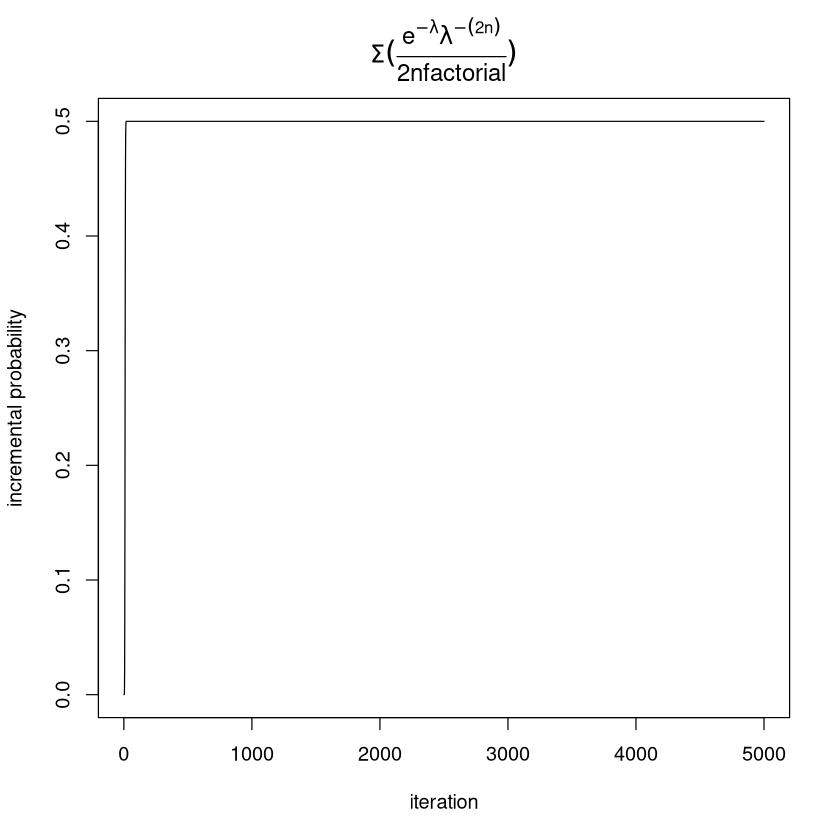
\includegraphics[width=10cm,height=10cm,keepaspectratio]{3c}

\caption{The incremental probability.}

\end{figure}


\section*{4-}

\subsection*{a)}

There are two distributions and both of them are binomial. The first
one is being able to vote or not and the second is voting for x or
y. Let the first distribution be $p(X)$ and the second $p(Y)$. Consequently,
the total distribution is 

\[
P(X=x)=\binom{n}{x}p^{x}(1-p)^{n-x}
\]

\[
P(Y=y|X=x)=\binom{x}{y}q^{y}(1-q)^{x-y}
\]

\[
P(Y=y)=\binom{n}{y}(pq)^{y}(1-pq)^{n-y}
\]

In this case, $P=0.5$ and $q=P$ then

\[
P(X_{A}=x)=\binom{N}{x}(0.5p)^{x}(1-0.5p)^{N-x},
\]
\[
P(X_{B}=x)=\binom{N}{x}(1-0.5p)^{x}(0.5p)^{N-x}
\]

Now that the probability of stheuccess is found, the mean value can
be estimated as:

\[
\frac{Np}{2}
\]

and the expected value of variance is $\frac{Np(1-p)}{4}$ and the
standard deviation is $\sqrt{\frac{Np(1-p)}{4}}$

\subsection*{b)}

As N reaches infinity, $\frac{N}{2}$ also becomes infinity. Then

\[
E[X]=p\times\lim_{N\rightarrow\infty}\frac{N}{2}=Np
\]

This is a number between $\left[0,N\right]$ to find the fraction
of students, $Np$ has to be devided by $N$ which will be equal to
$p$.

\subsection*{c)}

In section A the expected value of two binomial distributions which
are conditional was prove to be $nqp$ the second binomial is fixed
but the first binomial has changed.

The first binomial is the probability of voting if busy and supporting
A. its success chance is $0.25q_{a}$. Another scenario is voting
if free and supporting A which has a success of $0.75(1-q_{A})$.
These two probabilities have or between them. if two distributions
are ored, their distributions are summed and expectation of sums is
sum of expectations. Hence:

\[
E(X_{A})=0.25q_{A}pN+0.75(1-q_{A})pN
\]

By the same logic,

\[
E(X_{B})=0.25q_{A}pN+0.75(1-q_{A})pN
\]


\section*{5-}

\subsection*{a)}

Two disjointed events cannot happen at the same time but two independent
events can happen although the outcome of one gives no information
about outcome of the other

\subsection*{b)}

If two events (A,B) are disjointed such that P(A)=1 and P(B)=0 then:

\[
P(A\cap B)=0
\]
and 
\[
P(B|A)=\frac{P(A\cap B)=0}{P(A)}=0=P(B)
\]


\subsection*{c)}

If N is greater than 2(for example N=3):

IF A is true, then there can be 2 boys one girl or 2 girls and one
boy. For the first case, B is false and for the second case B is true.
Hence Truth of A gives no information about truth of B

IF A is false, then either the children are all boys or girls. The
former results in B being false since there are 3 boys and the latter
makes B true since there are zero boys. Therefore, falsehood of A
gives no information about B either.

\section*{6-}

The sample space is {[}bb,bg,gb,gg{]}

\subsection*{a)}

The mother's response removes ``gg'' from the sample space. Therefore,
the probability of ``bb'' is $\frac{1}{3}$

\subsection*{b)}

Like the previous section.

\subsection*{c)}

The name of the child gives no additional information reguarding the
problem. The question is only conserned with the children's gender.

\section*{7-}

\subsection*{a and b)}

Suppose there are N players. When two players meet in round k, they
are effectively the chosen 2 from a pool of $2^{k}$ players who competed
in the sub-bracket leading to that particular match. Let us call such
a sub-bracket a k-sub-bracket. There are $M_{k}=2^{N}/2^{k}$ k-sub-brackets.
The probability that both players end up in a particular k-sub-bracket
is

\[
P_{1}(k)=\frac{2^{k}}{2^{N}}\cdot\frac{2^{k}-1}{2^{N}-1}.
\]

The probability that two players from a k-sub-bracket meet in round
k is

\[
{\displaystyle P_{2}(k)=2\cdot\frac{1}{2^{k}}\cdot\frac{1}{2^{k}-1}=\frac{1}{2^{k-1}}\cdot\frac{1}{2^{k}-1}.}
\]

Thus, the probability that the two players play each other is

\[
P_{N}=\sum_{k=1}^{N}M_{k}\cdot P_{1}(k)\cdot P_{2}(k)=\sum_{k=1}^{N}\left(\frac{2^{N}}{2^{k}}\right)\left(\frac{2^{k}}{2^{N}}\right)\left(\frac{2^{k}-1}{2^{N}-1}\right)\left(\frac{1}{2^{k-1}}\right)\left(\frac{1}{2^{k}-1}\right)=\frac{1}{2^{N}-1}\sum_{k=1}^{N}\frac{1}{2^{k-1}}=\frac{1}{2^{N-1}}.
\]

for $N=4$ 

\[
\frac{1}{8}
\]


\section*{8}

\subsection*{a)}

There is a single outlier which ruins the plot at index 1429.

\begin{figure}[H]

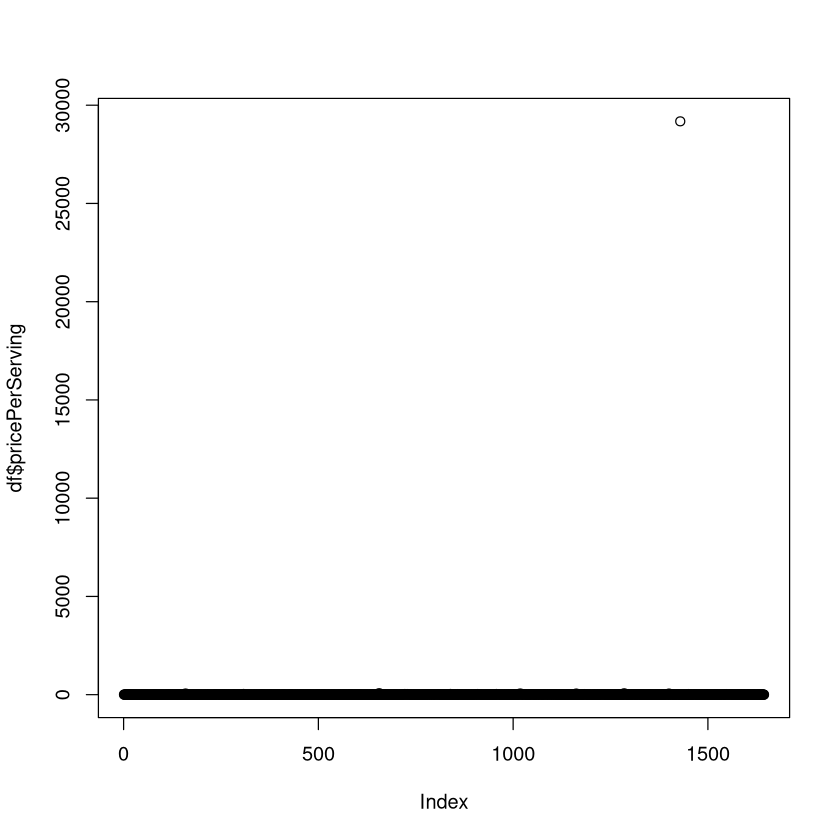
\includegraphics[width=10cm,height=10cm,keepaspectratio]{8afig1}\caption{outlier demonstration}

\end{figure}

After removing the outlier the plot looks like

\begin{figure}[H]

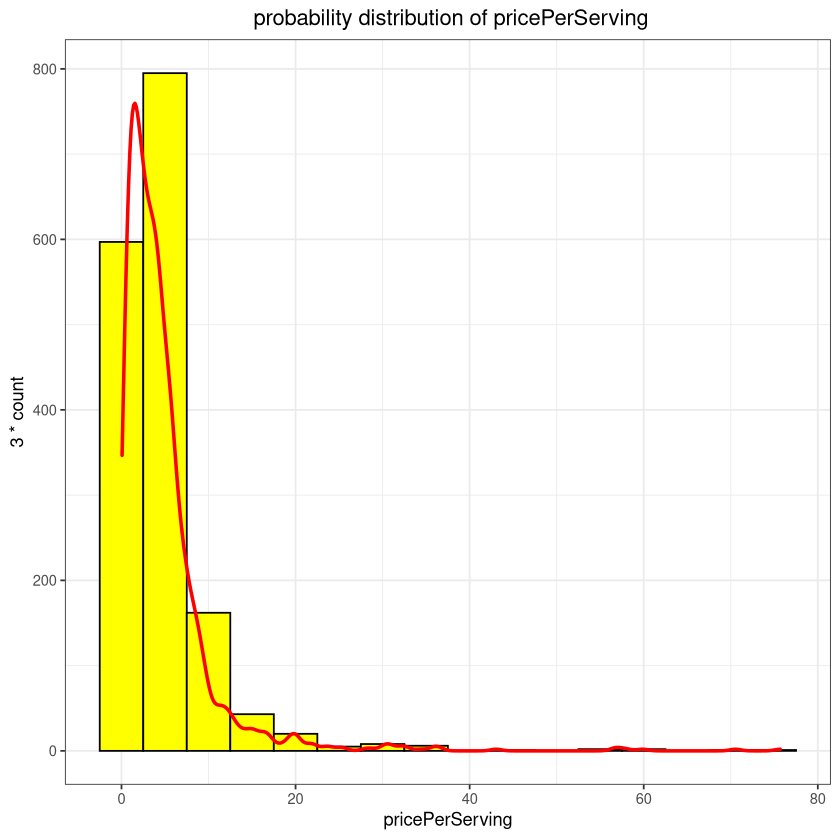
\includegraphics[width=10cm,height=10cm,keepaspectratio]{8afig2}\caption{Histogram of price per serving with density line}

\end{figure}


\subsection*{b)}

\begin{figure}[H]

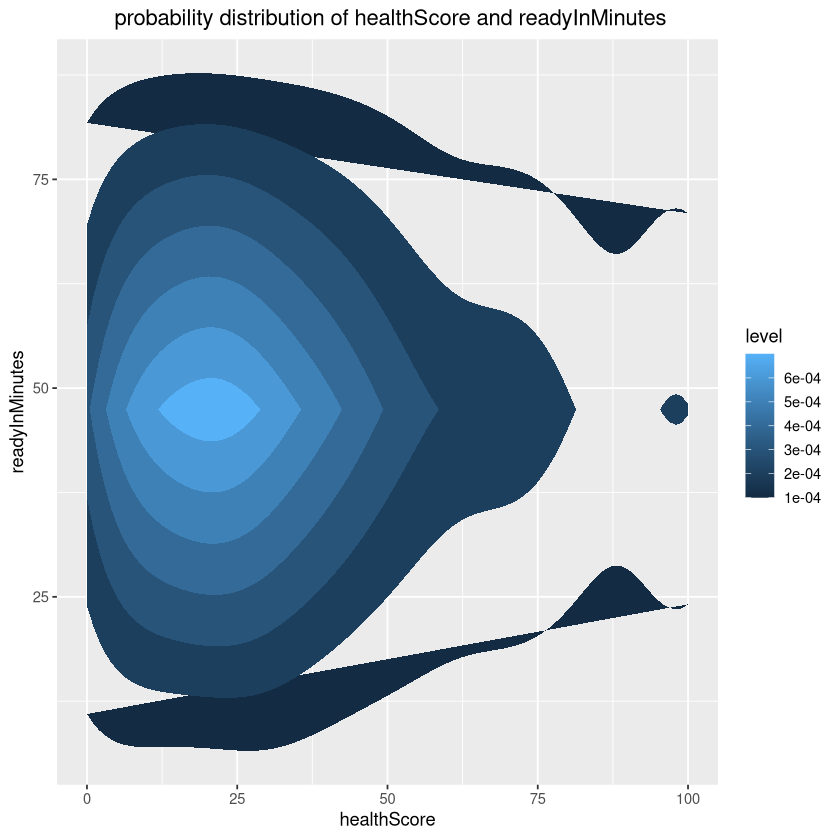
\includegraphics[width=10cm,height=10cm,keepaspectratio]{8b}\caption{probability distribution of healthScore and readyInMinutes}

\end{figure}


\subsection*{c)}

\begin{figure}[H]

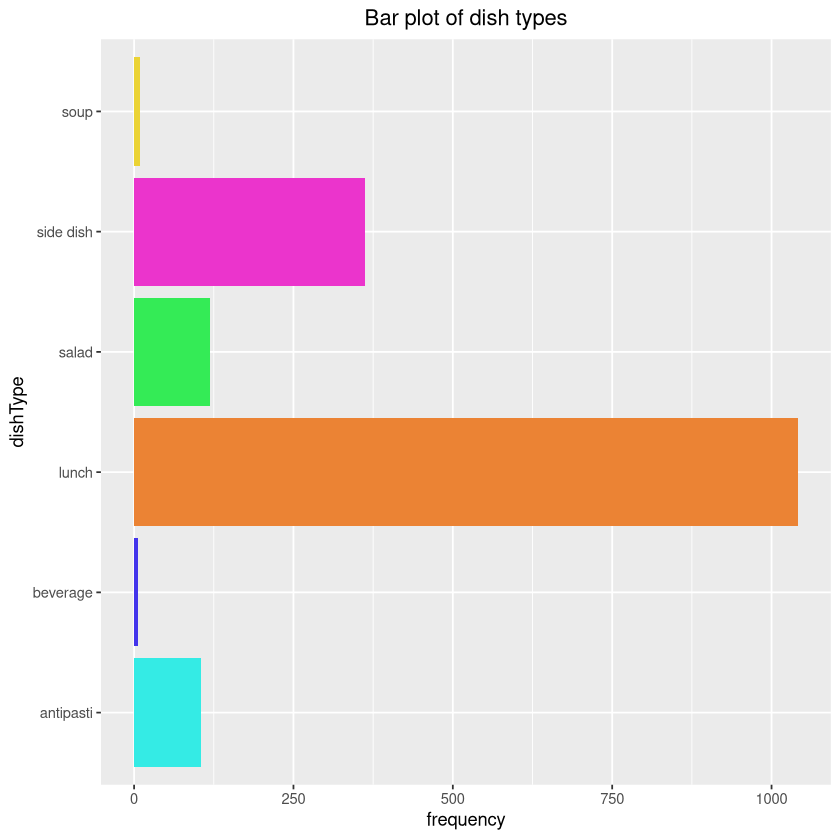
\includegraphics[width=10cm,height=10cm,keepaspectratio]{8c}\caption{Bar plot of dish types}

\end{figure}


\subsection*{d)}

\begin{figure}[H]

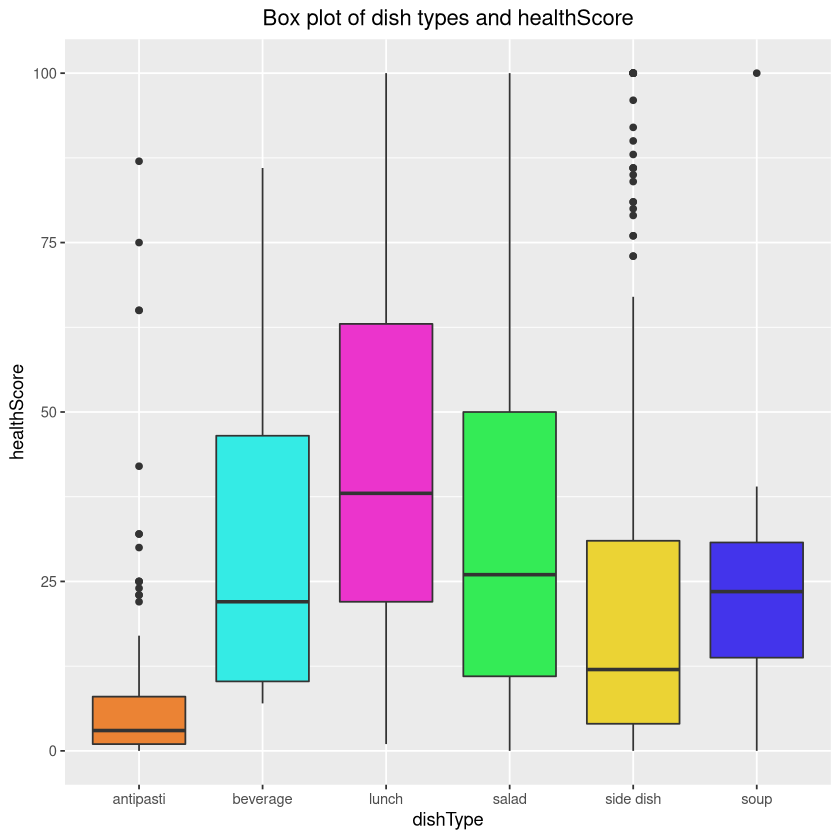
\includegraphics[width=10cm,height=10cm,keepaspectratio]{8d}\caption{Box plot of dish types and healthScore}

\end{figure}


\subsection*{e)}

\begin{figure}[H]

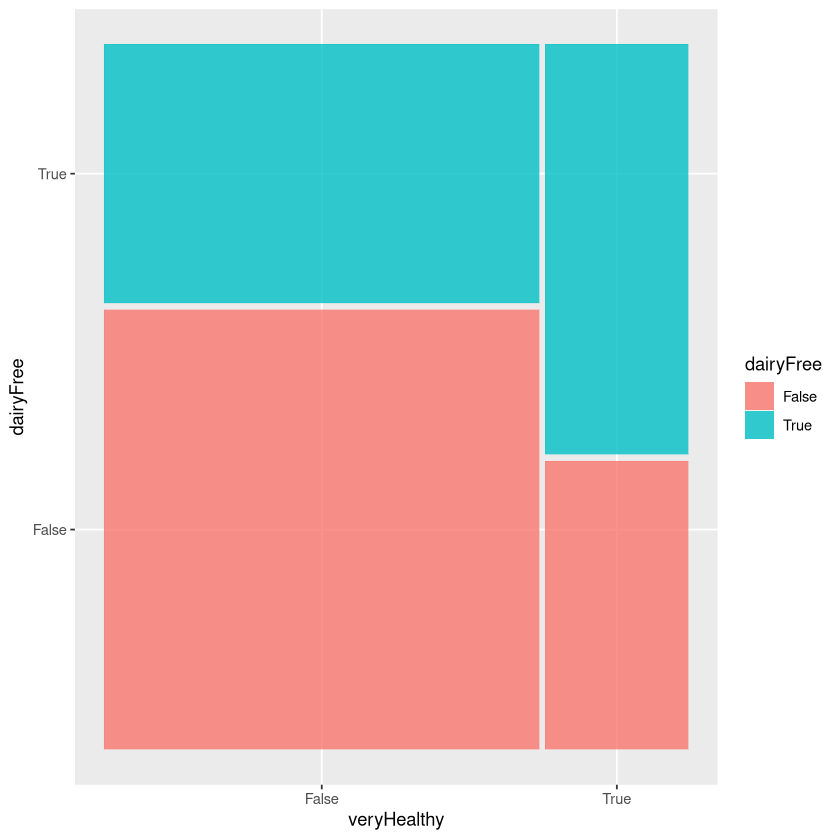
\includegraphics[width=10cm,height=10cm,keepaspectratio]{8e}\caption{mosaic plot of dairyFree and veryHealthy}

\end{figure}

\end{document}
